\documentclass{cmspaper}
\begin{document}

%==============================================================================
% title page for few authors

\begin{titlepage}

% select one of the following and type in the proper number:
   \cmsnote{2005/TBD}
%  \internalnote{2005/000}
%  \conferencereport{2005/000}
   \date{\today}

  \title{DRAFT Technical Design of the Dataset Bookkeeping System DRAFT}

  \note{Draft Version v0.8...}

  \begin{Authlist}
    M. Anzar Afaq, Lothar Bauerdick, Greg Graham, Vijay Sekhri, Igor Terekhov, 
    Yujun Wu
       \Instfoot{fnal}{Fermi National Accelerator Laboratory}
    Lassi Tuura
       \Instfoot{ne}{Northeastern University, Boston, MA, USA}
    Peter Elmer
       \Instfoot{prince}{Princeton University, Trenton, NJ, USA}
    Tim Barrass
       \Instfoot{bristol}{University of Bristol, Bristol, UK}
  \end{Authlist}

\collaboration{for the CMS collaboration}

  \begin{abstract}
      This note describes the Dataset Bookkeeping System (DBS) prototype for the 
  CMS Data Management (DM) project.  The DBS will
  store information about real and simulated CMS data in a queryable format. 
  The supported queries will allow users and their agents to discover avaliable 
  data, to retrieve further information about specific data, and to 
  derive datasets for use in analysis. This note contains some use cases 
  and requirements for the DBS.  The technical design of the DBS prototype
  is presented.
    \end{abstract} 

  
\end{titlepage}

\setcounter{page}{2}%JPP

\section{Introduction}
\label{sec:intro}

The Dataset Bookkeeping System (DBS) is part of the CMS Data Management system
and provides the means to discover, define and use for processing CMS event 
data. It tracks primarily {\em datasets} and their associated attributes.

This document describes the concepts used by CMS in data management and
specifies the bookkeeping system in detail that is sufficient to build the
baseline data management system described elsewhere~\cite{dmman}.  We begin
with a description of the CMS data organisation by expanding on the work of
the Data Management RTAG~\cite{rtag7}, the CMS Computing Model~\cite{CM} and
the CMS Computing Technical Design Report~\cite{CTDR}.
This is followed by a set of scenarios illustrating the primary uses of the
bookkeeping system.  Finally we provide a mapping of the organisational
concepts to relational database entities followed by an architectural
description of the components making up the bookkeeping system.

Access to CMS data should take place through interfaces designed for an 
appropriate level of abstraction for the end user.  The system will not require 
knowledge of implementation details, such as files or transport mechanisms. 
The dataset bookkeeping system (DBS) will take advantage of external infrastructure where 
possible.  The design will occasionally make 
reference to external databases or systems as required.  The DBS will 
concentrate on supporting the decomposition of datasets into event collections, 
finding the 
components needed to analyze or to transfer an event collection, and the making 
attributes available to support a sensible level of dataset discovery service.  

The main features that will be provided by the DBS are 
\begin{itemize}
\item Dataset Discovery.  The user should be able to present the DBS with 
interesting parameters describing data and retreive either a dataset or
a set of Event Collections satifying the query.
\item Dataset Creation and Characterization.  As a result of a query, the 
user will be able to store a dataset definition along with information 
characterizing the dataset.
\item Input for Parallelization.  Tools for building parallel jobs used in MC 
production, data reprocessing, and by users doing analysis will be able to use
the DBS to render information for parallelizing a generic request for processing.
This will take place behind the scenes without explicit user knowledge.
\end{itemize}

\section{Refining the Data Organisation}

\begin{figure}[hbtp]
  \begin{center}
    \resizebox{10cm}{!}{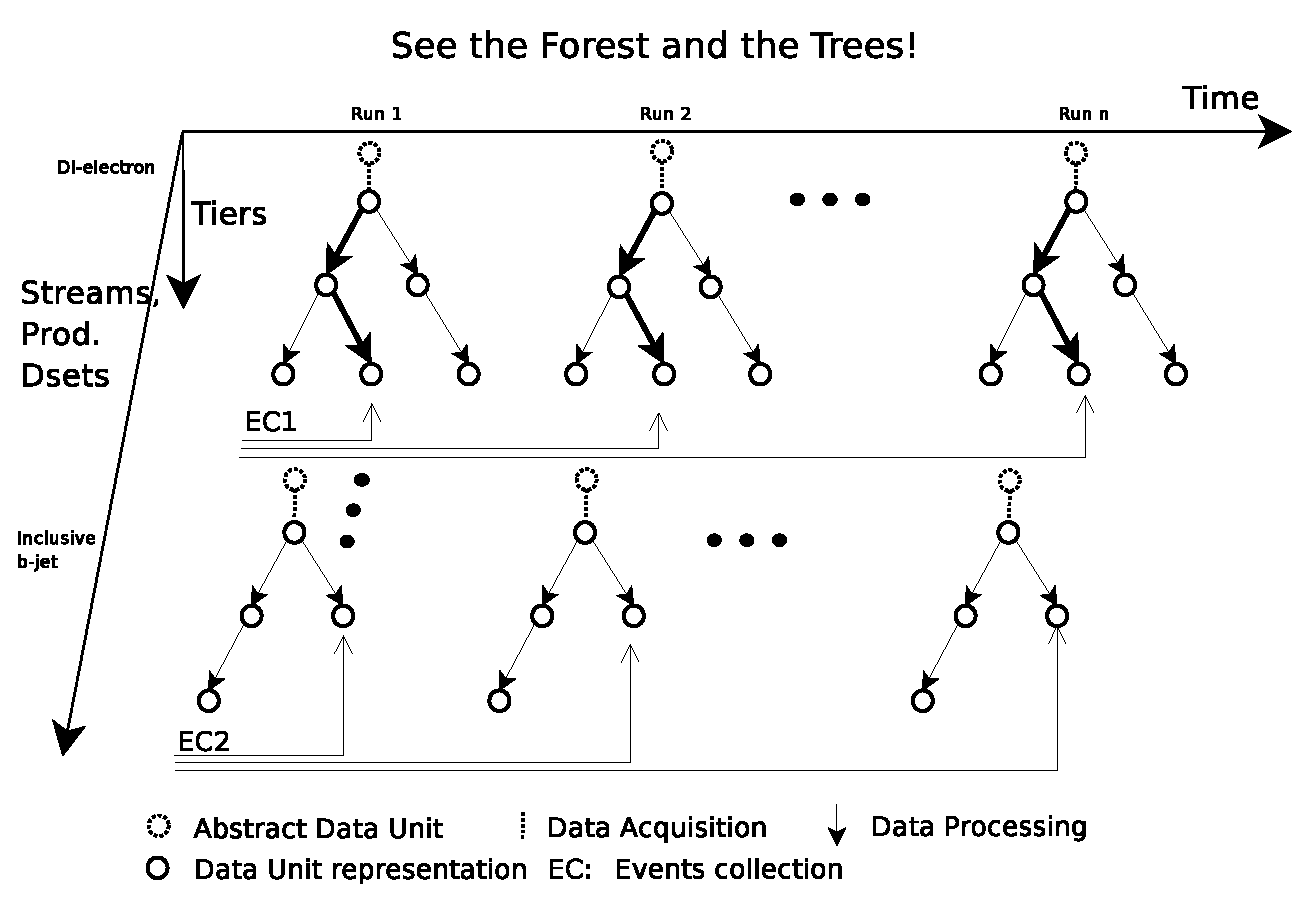
\includegraphics{forest.eps}}
    \caption{The figure shows a forest of trees.  The root of each tree is a 
chunk of data indexed by some number monotonically increasing along the time axis, 
such as run number or luminosity segment.
The path to a node in the tree from the root represents the result of processing 
the root node data through a particular sequence of processing steps.  Each node 
along the way corresponds to an intermediate step.  The individual nodes correspond to objects 
called Event Collections.  Along the axis pointing out of the page, the trees are 
indexed by the qualitative kind of data, or by Primary Dataset. The collection of all 
Event Collections at the same Processing Path within a Primary Dataset is known as a
Processed Dataset. (Exampled of Processed Dataset are unfortunately labeled here 
as "EC1" and "EC2".)}
    \label{fig:forest}
  \end{center}
\end{figure}

We following terms define the organisation of CMS data:

\begin{itemize}
\item {\bf (Online) Stream}.  A stream is the largest unit of data organisation
and can be thought of as a collection of the output event data from the CMS
detector grouped by sets of high-level triggers that roughly ``go together'' 
for analysis purposes. This plays a minor role in the DBS.

\item {\bf Primary Dataset}, also known as Production Dataset or Abstract Dataset. 
\footnote{Confusion arises in some quarters as to the meaning of "Primary Dataset", as 
it also connotes a dataset consisting of only Raw data. "Abstract Dataset" was proposed
as an alternative, but has not yet been adopted.} This is the the unit of 
data accessed to analyse a given trigger.  It contains data at all levels of 
processing pertaining to a given trigger or common MC production criteria.
Discovery and delivery of data is mainly concerned about primary datasets.
For real data CMS expects to have of the order of 50 primary datasets.  
For Monte Carlo data ``primary datasets'' comprise data generated with the 
same parameters.

\item {\bf Processed Dataset}. This is a slice of data from a Primary Dataset
defined by the exact processing history applied to it.  For example, the reconstructed data
processed with application A and version V and configuration C, and other cardinal 
parameters is a 
{\em processed dataset}, namely it is the result of processing the raw data.  The 
exactness of the Processed Dataset is needed because this is the way the DBS 
tells Event Collections apart if they have the same run number of luminosity 
segments and yet different software versions produced them.


\item {\bf Data Tier}. This is the type of content resulting from a 
degree of processing applied to the data: {\em RAW} The raw event data 
written by the filter farm; {\em RECO} All reconstructed data coming from 
the production engine; {\em FEVT} RAW + RECO; etc. In practice, this is essentially
like the Processed Dataset in that it is a slice of data from a Primary Dataset 
defined by processing level, but it is a thicker slice.   By design the 
Data Tier ignores distinctions between exact processing histories and 
configurations where the user deems those distinctions unimportant.  For example, 
if a minor change is made to the reconstruction code that is not deemed 
important enough to go back and reprocess a hundred terabytes of data, then 
the new code will produce data at the same Data Tier but at a different 
Processed Dataset.  (The user will know about Data Tier- the Processed Dataset 
will be used internally.)

\item{\bf Event Collection}. The smallest subset of a Processed Dataset that
user is able to access through the bookkeeping system without using an
analysis application.  The Event Collection is indexed by some externally 
provided number, such as run number of luminosity segment, and it maps to 
one or more files.  These are the data management atoms that 
the user has to play with.

\item {\bf Analysis Dataset}. A user defined collection of Event Collections 
within a Data Tier.  This may in general span multiple Processed Datasets 
differing by no more than a minor difference in the Data Tier sense, but 
it will not allow duplicate Event Collections in run number nor mixing of 
Event Collections from different Primary Datasets.

\item {\bf Run}.  A run is a well defined index used in HEP experiments to 
catalog data by time interval. The run is generally associated with quality 
parameters and a rough luminosity estimate and with specific sets of calibration
constants.

\item {\bf File}  The file reflects the physical container for the data.  It is
an implementation detail which will be hidden from the user.  An N to N file 
mapping with Event Collections is allowed, and a file is allowed to span 
multiple Event Collections in order to support legacy cases.  In the future, 
constraints may be applied to the data model here.

\end{itemize} 

We present these entities in Figure~\ref{fig:highlevel}.  
The figure expresses the basic unadorned information model
for the bookkeeping system, not the actual schema we will use.
The mapping of the information model into a schema is discussed in more
detail in section~\ref{sec:details} after we have listed some primary use
cases.  A more precise definition of these entities in terms of subsets of
the data appears in the Appendix~\ref{appendix}.

\begin{figure}[hbtp]
  \begin{center}
    \resizebox{9cm}{!}{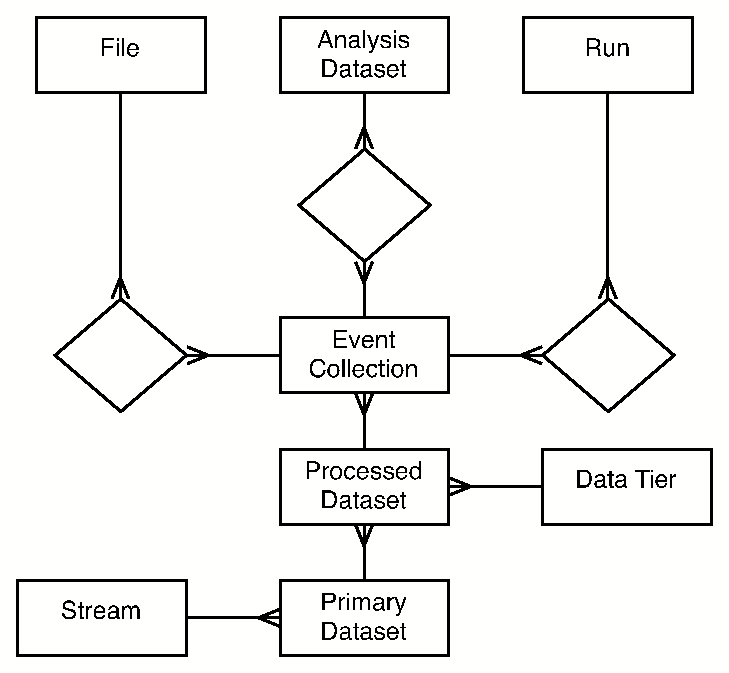
\includegraphics{DatasetBookkeeping-new-1.eps}}
    \caption{Basic outline of the core DBS schema including the basic entities outlined 
above: Primary Dataset, Processed Dataset, Data Tier, Event Collection, Analysis Dataset, Run, 
Stream, and File.  Three mapping tables are required for N to N relationships of 
Event Collection to each of Analysis Dataset, File, and Run for a total of eleven "core" tables. }
    \label{fig:highlevel}
  \end{center}
\end{figure}

\section{Implementation Concepts}

The Dataset Bookkeeping System contains the following implementation concepts 
that will be hidden from the users.  

\begin{itemize}
\item Files.  Although File is also a core concept, it is one that should be hidden 
from the user.  The DBS contains names of logical files and not physical files or 
locations.  It is not yet
determined how much file level metadata will be tracked by the DBS, but this could include 
size and checksum information.
The DBS will treat special files, such as ``META'' files, in 
exactly the same way as all other logical files.  Special files that 
appear in more than one Event Collection will appear in more than one
relational row.  However, the EDM group will 
make changes in the way data is written in CMS so that the number of 
such special files tends to zero in the long run.  
\item File Blocks.  The DBS contains Blocks as special aggregations of Event 
Collections. Blocks are aggregations with respect to underlying 
infrastructure optimized for efficient storage and transfer.  The Data
Transfer system is expecting that the File Blocks will be expressed in terms
of files.  However, the DBS will store these as blocks of Event Collections and then 
a simple query can be done to retreive the list of files as needed.  We assume that
we will never want to ship a file that is a fractional part of an Event Collection
without the other files in the event collection.  This adds a single table that is a 
subtype of Analysis Dataset.  (Another table is needed to track subtypes.) 
\item Application Parameters.  The DBS will contain p[arameters that are deemed interesting
for user queries so that the users can find data.  The early identified "important" parameters
such as number of events and estimated luminosity will be stored on table with the Event 
Collections and Analysis Datasets.  However, we anticipate missing some interesting parameters
to start out with, and we also anticipate users wanting to store parameters of interest to 
specific users for later queries and not general interest parameters.  In the latter cases we 
envision a generic parameter system that is somewhat slower to query but much more flexible in 
what it can store.  These may include parameters marked as "queryable" 
from the framework, for example.  
\item Parentage Tracking and Compositeness.  Parentage and Compositeness can be added on an
as needed basis to selected entities with a simple ER 
design pattern of adding an N to N self-mapping table.  We envision that Analysis Datasets
will need to track parentage since the API supports this, we also envision needing to track 
parentage among Event Collections where filters and skimmers are processing multiple Event 
Collections into one, and we envision possibly needing to track compositeness of Event Collections
across Data Tiers (ie- the "RAW+REC" composite datatype.)   This accounts for three more tables.  
\end{itemize}

\subsection{More Information on Application Parameters}

All general purpose parameters in the DBS are kept in String key/value format.  A 
Parameter Binding entity keeps track of specific key/value pair bindings, while a 
Queryable Parameter Set groups related bindings together. (The Parameter 
Binding table can have duplicates to avoid the overhead of an N to N mapping table 
here, since a key/value pair can obviously belong to more than one parameter set.) 
An Application is described by a single table containing application name, version, 
and edxecutable name.  Finally, the mapping table of Application to Parameter Set is 
the Application Configuration.  It is instances of the mapping which are tracked 
in the Processed Dataset. This leads to five more tables, plus any small support tables.
These are shown in figure~\ref{fig:appl}.

\begin{figure}[hbtp]
  \begin{center}
    \resizebox{9cm}{!}{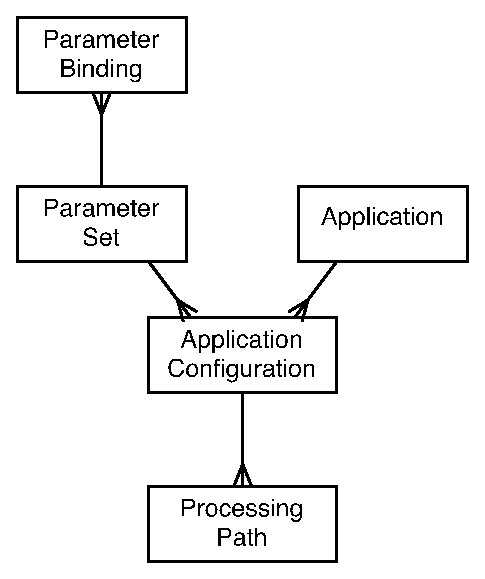
\includegraphics{DatasetBookkeeping-new-2.eps}}
    \caption{Basic outline of the application and parameter tracking parts of the schema. }
    \label{fig:appl}
  \end{center}
\end{figure}

\section{Scenarios, Use Cases, and Example Queries}

In this Section, we explore data import
({\em putting} data into the system), queries ({\em seeing} what is there),
and workflow for read access ({\em getting} data out of the system).

\subsection{User Queries}

Below we explore user queries corresponding to the various access modes,
and subsequently attempt to generalize. Among the goals of this section
is clarification of the role of a ``run''.

\subsubsection{Use case 1: Detector Expert}

  The first use case for selecting on run is doing detector studies, calibrations
and data quality. This use case does not address the time-varying 
calibrations/conditions are stored and accessed by applications from the 
conditions database itself, but merely how someone doing such studies would 
find the event data to do such studies. The common paradigm in HEP to access 
data through runs.
\begin{itemize}
\item An expert coming in the morning, reading the logbook sees that there was
     some problem with their subsystem overnight in run NNN; for example, if a crate 
     tripped off or was in some strange state, or oddities were seen in some 
     monitoring histogram, etc. Then the expert wants to look at some raw or 
     reconstructed data with some specialized application to learn more about the
     run quality or problems, often to classify it in a data-quality sense.
\item The detector expert at some later date may try to determine
     some calibration constants or corrections. Also in this case it will be natural
     for the expert to ask for different types of data, most typically with
     run ranges. Often what they do may include one component of actually 
     trying to break up the data into run ranges based on the problems and
     state of the detector and one component of actually determining the
     calibrations. 
\end{itemize}

``Run'' here represents a natural quantum for thinking about the problem and
the DBS will be asked for data in these terms. Two implications are:
\begin{itemize}
\item The DBS will be asked for data at any tier from particular
    primary datasets with ``run'' as a selection. This has to be supported and
    some means of configuring jobs at this granularity for at least these
    categories of data must be provided.
\item ``Data quality'' attributes are likely 
    to be specified with a granularity of a single run. These flags may be
    specified for all data tiers of a particular run's data or just
    for particular ones. 
%    (As part of the discussions of the details of how
%    ``run'' is defined, DM should bring this point up explicitly. As it is a 
%    relatively common model in HEP, we can probably assume it for the moment.
%    See below for further details.)
\end{itemize}

Runs can be represented as Event Collections, and run numbers can be stored 
in a metadata support table going along with Event Collection.  Querying on 
run number amounts to first querying on attributes that can identify a 
Primary Dataset and a history of Processing.  Then by providing the set of 
interesting run numbers the corresponding Event Collections can be found.

The fact that data is accessed by ``run'' does not imply that the 
calibrations or conditions need to fall on run boundaries.  Up to a few 
parameters of interest for querying, these are usually 
read in bulk by applications so that there is no need to track these in the 
DBS.    Simple attributes like Run status flags 
can be stored in the DBS and later queried 
if they are imported along with the Event Collections.
Similarly data quality decisions with a finer granularity than 
run will be handled by an external conditions database and require 
the use of an application for access. 

\subsubsection{Use case 2: Production}
\label{sec:UCprod}

  The production system typically takes an Analysis Dataset or Processed Dataset
as input and processes it to produce a processed representation the input, or 
another Analysis Dataset or Processed Dataset. This use case includes reprocessing
and Monte Carlo production.

%  So how are ``runs'' sometimes used here? 

\begin{itemize}
\item The input Analysis Dataset is specified by a run range or list
     of runs, most likely made by selecting on data quality attributes set by
     someone like the expert of use case 1.  
%\item If the output is intended to be selectable with a run granularity,
%     the production system may process a given dataset by 
%     breaking it up into individual pieces with a granularity such that
%     the run genealogy of each output can be followed back to an input.
\end{itemize}

The user may be interested in tracking two types of ``history'' here:
\begin{itemize}
      \item macro level: how one dataset was transformed to another
      \item micro level: how one ``run'' representation is mapped to anther one
\end{itemize}
The first is tracked by explicitly including the processing path in the
definition of an Event Collection as represented internally in the DBS.  
The second is tracked by maintaining a relation between Analysis Datasets
and Event Collections.

The use of run ranges and/or run lists explicitly to define the input is 
partly incidental. If the goal of the production system is seen as
processing one dataset into another, the run-ranges and/or run lists 
should be captured explicitly in the DBS as an Analysis Dataset. 
%I would claim that the proper 
%concept for capturing this is a ``dataset'' (e.g. as some sort of ``dataset 
%tag''). 

If the output is intended to be queryable by run number, then the production 
system may process the input dataset by breaking it up into runs.  This is the 
easiest scenario to envision because the processed runs can then be stored 
directly back into the DBS and aggregated into an output Analysis Dataset such
that input runs and output runs are in one to one correspondence.
However, even the hard case involving splitting and merging can be represented here. 
See section \ref{sec:createEvColl} for more information. 
The production system is explicitly collaborating in propagating the
``run'' granularity from input to output.  It can choose any granularity it 
wishes as long as it is tracked by the DBS.  

Otherwise, this use case is supported in much the same way as the previous one.  An input 
Primary Dataset and input processing path is given, and then all Event Collections
matching the run range can be retrieved.  When tracking the processing
taking place within a Primary Dataset, even if the framework does not track processing
of individual Event Collections within an Analysis Dataset, the Event Collections 
may be loaded into the DBS anyway.  This preserves the structure of tracking 
the processing paths through Event Collections, and the set of 
files corresponding to the whole processed Analysis Dataset can be assigned to 
each Event Collection in the derived Analysis Dataset.  

\subsubsection{Use case 3: Analysis End-user}

  The analysis end-user will process Analysis Datasets for more
than one run through some application such that the output no longer has
a 1-1 mapping to run. See section \ref{sec:createEvColl} for an 
explanation of how such filter and skim output can be 
represented in the schema.
\begin{itemize}
\item The detector expert is still working and may decide, after the 
     analysis-user has already run their analysis over a dataset, that a
     particular run was ``bad'' after all and should be excluded from their
     end result. 
\item The detector expert or analysis group may provide some set of
     corrections/updates which the analysis-user needs to apply themselves
     For example, constants that arrive too late to be included in 
     the last re-reconstruction or AOD production step, or were 
     actually generated from the output of
     the last re-reco or AOD production step. 
\end{itemize}
The DBS and DM should be involved in tracking Analysis Datasets in which
some mangling has gone on with respect to runs and the relationship of 
the resulting Event Collections to runs becomes significantly more complex.

In the case 
where multiple jobs are doing the processing, the DBS should also be able
to keep track of which expected data units have been imported successfully and which 
have not.  In the case where there is only output product Analysis Dataset, 
then it is still useful to be able to query and find out which component
input Event Collections, it doesn't matter were processed to 
arrive at the desired result.  This is important to be able to track important 
aggregate dataset properties like luminosity.

\subsubsection{Workflow scenario}

The following workflow building scenario explores the 
interface between data management and workflow management.
\begin{itemize}
\item A physicist or agent creates jobs based on data identified by queries against 
the DBS.  A handle to an Analysis Dataset containing a number $N$ of
Event Collections is returned.  
\item The physicist or agent creates $M \le N$ jobs.  The agent may create jobs with more than 
one Event Collection per job if optimization works out that way.  The job 
creation tool creates jobs in a site-independent fashion, knowing only about 
site-independent dataset parameters, input event collections, etc 
\item Physicist or agent submits jobs. Job submission tool consults the DLS. 
Information about sites where the data resides is obtained now. Some element
of the workload management system (e.g. the resource broker for LCG) will
decide on which site the job may run.

\item Job files are transferred to the execution site along with the job 
\item The jobs are 'localized' upon transfer to the site. 
\item Output data is created by the job. The job consigns this data to
some storage at the site where the job ran. A data transport system may
subsequently (and asynchronously with respect to the job ending) move that 
data to some other final location.
\item The output data is published into the DBS.
\end{itemize}




\subsection{Introducing Dataset Pathnames}

  The Dataset Bookkeeping System will support an API that hides the details of the 
schema objects from the user.  The objects exposed to the user include Primary Dataset, 
the Data Tier, the Event Collection, and the Analysis Dataset.  
The first three of these objects represent dimensions that identify the data 
according to physics kind, processing history, and sub-unit 
(ie- "run number" or "lumi section") respectively.  The forth object represents an 
aggregation of Event Collections into system defined or user defined sets.  

  The object of immediate interest to the physicist is however the Analysis Dataset.
Except for bookkeeping purposes, the physicist is uninterested in the substructure
of individual Event Collections.  Therefore the API should support this abstraction.
However, it is still natural for the physicist to request the data in terms of 
kind and processing history.  This suggests that the thing a physicist carries 
around to identify his/her data has three components: the Primary Dataset Name, the 
Data Tier Name, and the Analysis Dataset Name.  
\begin{equation}
     \mbox{Data Identifying PathName} = /PD/DT/AD
\end{equation}
where $PD$ is the Primary Dataset, $DT$ is the Data Tier, and $AD$ is the Analysis 
Dataset.

  This pathname can be mapped easily onto the tables as defined so far.
The API should hide the details about Event Collections 
unless needed specifically to build or dump the contents of an Analysis Dataset.
The API should also hide the details about the parentage relationships among 
Event Collections and Analysis Datasets.  For example, if $AD_1$ is fully processed 
into $AD_2$, then the pathname to $AD_2$ is just $/PD/DT/AD_2$ and not 
$/PD/DT/AD_1/AD_2$.

  The API methods needed to manipulate Analysis Datasets may include: 
\begin{itemize}
\item addEventCollection( basePathName, ECInfo ) 
       where basePathName is the $/PD/DT$ part of a pathname, and ECInfo 
       is a structure containing required and extra parameters for describing 
       the Event Collection, including the luminosity estimate, run number, 
       number of events, and list of files.  (Possibly also lumi segment 
       information, see below.) 

\item pathName = buildDataset ( basePathName, $AD$, list<EventCollections> )
       where basePathName is as above, $AD$ is the desired name of the new
       dataset,  and list<EventCollections> is a list of Event Collections in 
       terms of some yet-to-be-named identifier.  (The point is to have an API 
       that builds directly from a list.)  If $AD$ is already a name used 
       somewhere else, this will generate an exception.   (We can introduce 
       namespaces later to help avoid conflicts.  On success, the pathName should 
       be returned as the basePathName + / + $AD$.) 

\item  pathName = buildDataset ( initialPathName, $AD$, predicate )
       If initialPathName is a basePathName as above, then $AD$ and pathname 
       are also as above, and the list of Event Collections is generated by a
       query from among all the Event Collections in /PriDName/ProDName matching 
       the given predicate.  If initialPathName is itself an Analysis Dataset, 
       then the predicate is evaluated against only the Event Collections in the
       Analysis Dataset.  The returned pathname will drop the basename of the 
       initial path and replace it with the new $AD$ so the the returned path 
       still has a depth of three.  

\item  list<EventCollections> = displayDatasetContents ( pathName ) 
       This provides a list of event collections in an Analysis Dataset 

\item  list<EventCollections> = displayDatasetContents ( initialPathName, predicate ) 
       This provides a list of event collections satisfying a predicate as in 
       buildDataset above.  (This method is intended as a helper for 
       buildDataset.) 

\item  pathName = buildDataset ( basePathName, $AD$ )
\item  closeDataset() 
       It is intended that Analysis Datasets are normally "snapshots" of the 
       available data at a particular time.  Therefore the API methods defined so 
       far will create and close Analysis Datasets while recording information 
       internally about the API call that created them, including the timestamp,
       the initial query if present and the parentage if created from another 
       Dataset.  Workload management needs to be able to create open datasets
       and add Event Collections to them as they become available.  Therefore  
       buildDataset with only two arguments will create an empty open Analysis 
       Dataset, and a special close call is provided to go along with it.
       These methods are only intended for local scope DBS. 

\item  addToDataset ( pathName, list<EventCollection> )
       This adds Event Collections to the already existing dataset given in 
       pathName.  These will be checked for consistency with the existing 
       Event Collections already there.  This method only works for 
       open Datasets in local scope DBS.
   
\item  globalPathName = publishDataset ( pathName )
      This method publishes an Analysis Dataset from a local scope DBS to the 
      global scope DBS.  The pathName is the full name of an Analysis Dataset in 
      local scope, and if it is also unique in the global namespace, then the 
      returned globalPathName is the same as pathName.  If the pathName is not 
      globally unique, then it is modified by the global scope DBS to make it 
      unique (ie- like appending an ordinal number to the end.) The local scope 
      DBS will make a note of this global name.  This method obviously must have
      concurrency controls at the point of contact with global DBS.

\item  deleteDataset ( pathName, deepFlag ) 
      This method removes an Analysis Dataset from the local scope DBS.  It will 
      be disabled at global scope.  If deepFlag is set, then the included Event 
      Collections that do not also belong to another Analysis Dataset at local 
      scope are also deleted.  Otherwise, all EventCollections are left in place.
\end{itemize}

Several helper API methods are needed to support the above.  

\begin{itemize}
\item  createPrimaryDataset ( /PriDName, PriDatasetInfo )
\item  createProcessedDataset ( /PriDName/ProDName, ProDatasetInfo )
      These create Primary and data tiers with appropriate data structures.
      For example, Primary Dataset needs to have some generator information in the 
      case of Monte Carlo and Trigger Path information in the case of real data.
      Data Tier needs to have Application information and parameters. 

\item  showDatasetInfo ( outputSelector )
      This method shows the metadata associated with an Analysis Dataset in desired
      detail by outputSelector.  It will include the query and timestamp as will as 
      contents.  In the case that the Analysis Dataset was built from an existing 
      Analysis Dataset, then the parent will be shown.  (Note: absolute parentage 
      in the sense of processing is kept at the Event Collection level.  This 
      parentage is purely logical and is only an artifact of possibly having built
      an Analysis Dataset from another in the buildDataset API method().)  It should 
      also show accumulated data like number of events and luminosity sum.
\end{itemize}

The relationship between Data Tier and Analysis Dataset can be made ORCA-like. 
For example, the special path $/PD/DT/DT$ can be taken to stand for 
all of the Event Collections in the Data Tier.  This will help hide further
the schema details from the user.   This special dataset will also have the special 
property that it can be open even at the global scope DBS.  This is to enable streaming.
As online publishes Event Collections into the global scope DBS, and we want to make 
them immediately available despite the fact that more are coming.

The Data Tier may properly contain duplicate Event Collections from the 
results of different processing paths that are not quite different enough 
to escape from the same Data Tier. In lieu of the final Data Tier specification
above, one can specify the exact Processed Dataset or Version, $/PD/DT/XV$ (where $XV$ 
stands for exact version) or just $/PD/DT/\mbox{Latest}$ for the latest and greatest version.

\subsection{Data import}

Data will be imported into the system in terms of the 
Event Collection entity.  

Even though data will be produced one file at a time, its import  
into the data management system is best done in terms of the 
more abstract Event Collection entity, because there will 
never be a case where files are useful outside of their event collection. 
We imagine the following scenario to put  a Event Collection 
into the system in such a way that supports streaming.

\begin{itemize}
\item An agent is in possession of a file or files associated with an Event Collection
containing real data.
\item The agent utilizes an API method addToDataset(*evCollInfo).  The evCollInfo structure 
will contain information like 
\begin{itemize}
\item Logical Filenames associated with the import
\item Attributes associated with the production of the Event Collection, 
including the latest processing step and the input Event Collection(s). 
\end{itemize}
\item The method searches for the best block to which to add the Event Collection.  
The ``block'' is a special Analysis Dataset envisioned for this purpose.  
\footnote{Blocks will have attributes of interest to a data transfer and storage 
system, like maximum size and location information. These are of system interest only.}
It should reconcile the processing history with existing processing paths and 
open a new Processed Dataset if necessary.
\begin{itemize}
\item If there is an open block, the Event Collection is added to the open block.
\item If there is no open block, a new open block is created and the Event Collection is added to that one.
\item If the new block size is greater than the maximum block size, then the block is closed.  
\end{itemize}
\end{itemize}

This is one simple algorithm that is ignoring local versus global scope DBS.  
There are many possible algorithms.  (FIXME)


\subsection{ Event Collections and Luminosity Estimates}

  There are two points to consider with regards to luminosity.  First of all, the 
standard index according to which "like" data is aggregated may be the index of
luminosity segments instead of run number.  There may be several luminosity segments 
per Event Collection, and summing them may be the mechanism by which luminosity
is assigned to the Event Collections in the DBS.   Secondly, the DBS should support 
dataset discovery in terms of luminosity.  Luminosity should be carried forward 
through subsequent processing steps of Event Collections, even in cases of skims and 
complicated N to N parentage relationships.  (This is possible with the existing 
schema.)  By carrying this information forward, it is possible to make this part 
of the API.  

  Consider the use case where the physicist is not interested in processing an 
absolute number of events, but rather is interested in processing some number of
inverse picobarns of data.
\begin{itemize}
\item  list<EventCollections>, foundLumi = partialDataset( pathName, lumiDesired )
       This returns a list of the first N event collections such that the sum 
       of their luminosity is the minimum luminosity above lumiDesired.  Also 
       returned is the found luminosity.  If there is not enough luminosity in 
       the given Analysis Dataset, then all Event Collections are returned.  The 
       user can check for this by checking foundLumi < lumiDesired.
\end{itemize}

Note that this can be combined with buildDataset() to create a luminosity "snapshot" 
within an Analysis Dataset.  In the case alluded to above, creating a snapshot of an 
"open dataset" is a way of providing a stable point of reference for analysis when 
data is being streamed into the corresponding Data Tier. For example: 
\begin{equation}
   /PD/DT/AD = \mbox{buildDataset} ( /PD/DT/DT, AD, \mbox{partialDataset} ( /PD/DT/DT, lumiDesired )[0] )
\end{equation}
could create a "snapshot" of interesting that doesn't change as more Event Collections
are being added to the special $/PD/DT/DT$ Data Tier.


\section{The Entities and Relationships}
\label{sec:details}

The schema can be logically divided into three sections.  First, the core entities 
shown in figure~\ref{fig:highlevel} support the core bookkeeping use cases of the 
DBS.   Second, the application and parameter related tables shown in figure~\ref{fig:appl}
represent a second distinct subsystem supporting different use cases. Finally, there 
are many support, auxilliary, and subtype 
tables that keep track of enumerations, descriptive data, and special dataset constrainst 
respectively.
These are described in thsi section and should be considered the most fluid and easily 
changeable class of schema elements.

\subsection{Adding More Detail -- Relations and Constraints}

The fundamental unit of data import into the system is the Event Collection.  A Event Collection 
can correspond to a run or any other chunk of data that is considered fundamental and can be 
mapped to a set of files\footnote{The set of files in one Event Collection are allowed to overlap with 
those in another Event Collection.  This accommodates metadata files, for example.  This 
aspect can be tightened later as the EDM evolves.}.  
A special kind of Event Collection is the Primary Event Collection.  The Primary Event Collection
corresponds to the root node in a processing tree of figure \ref{fig:forest}.  This entity
will contain attributes associated with the whole tree, possibly these are keys into 
an external Monte Carlo request database or run conditions database.

Analysis Datasets can support different kinds of constraints depending on the 
subtype.  The block would be a partition on Processed Datasets, and would have a 
relationship to a site entity.  
The block will aid in managing physical placement and storage of data.  
Blocks are therefore distinguished by having a one to many relationship to a supporting site 
entity.  Blocks satisfy the extra constraint that they  
partition the Processed Dataset\footnote{Technically, they partition the 
Processed Dataset in the sense that no event IDs
can exist in two different blocks.}.  This  simplifies the task of deciding which 
blocks to transfer given a set of interesting Analysis Datasets.

Blocks are special in that they represent a new implementation detail 
that must be hidden from the physicist.  However, block constraints and 
behavior can be hidden in the application layer.  Blocksize 
introduces a scale into the system,  however this can be addressed hierarchically 
through the self relation of Analysis Dataset
\footnote{If one introduces blocks in order to deal with data on a given scale, one someday may need 
to introduce ``super-blocks'' if that scale changes, and so on.}. 

User collections directly support the idea that users can specify 
collections of interest to them.  User collections list component Event Collections
and pre-existing Analysis Datasets and can span multiple blocks.  
envisaged.  The data associated with a RefDB production assignment can also be supported 
as a special kind of user collection.

A further specialization is the Snapshot.  The Snapshot is an Analysis Dataset whose results 
comprise the result of a query of the DBS.  The query itself is stored in a support table, and 
the cretion time is recorded.
The snapshot could be a closed set of Event Collections in a streamed dataset that does 
not change or grow as the dataset grows.  

The file entity contains obvious 
file attributes, such as logical filename, file size, cardinal times like creation and 
last access times, and checksum.  It does not contain site information or physical filename 
information.  Rather, replicas will be tracked externally.  

Event Collection will contain brief and essential attributes such as run number, 
number of events in the collection, cardinal times like creation and access times, 
and a run status flag.  Run conditions and calibration constants will
be kept in external databases.  Part of the primary key of the Event Collection
should be the Primary Dataset that the Event Collection 
belongs to as well as the complete processing path.  This should be a unique key of 
Processed Dataset.  

Blocks will have a unique block id that identifies its partition within its processed dataset.
It will have a block size and other low level attributes related to implementation.  Blocks 
will not contain physics metadata.  
Blocks will have a flag to indicate whether or not they are open for writing. 
In order to simplify the problem of locating blocks to sites, it is a 
requirement that open blocks be restricted to a single site\footnote{This has obvious 
implications for streaming, and can be later dropped or revisited when we review the distributed 
aspects.}.

The Processed Dataset will contain Primary Dataset and Processing Path 
references.
In addition, quantities that are determined to be ``searchable'' that are related to the 
specific level of processing of this data should be included directly here for 
users to query on.  

Analysis Datasets can contain further attributes.  User collections should for 
example contain annotations indicating why they were created.  Blocks contain 
pointers to sites.  Collections corresponding to assignment IDs will contain pointers 
into the RefDB plus some metadata for querying. Snapshots will contain references to the
text queries that created them.

Storage of attributes supporting the various 
entities  can be implemented as support tables when the actual schema is written down.  
The support table 
is a basic ER design pattern which allows metadata to be stored in a queryable format 
outside of the table directly representing the entity.  Attributes such as generation and 
simulation parameters for Monte-Carlo to run status information can be kept in support 
tables.   The support tables for the proposed schema have not been drawn for simplicity.  
Each principal entity in the schema should probably have a support table.

\subsection{Creating an Analysis Dataset from another Analysis Dataset}
\label{sec:createEvColl}

We examine a few cases here to illustrate how complex processing results can be 
recorded using the DBS schema.  
In general we think of Event Collections being processed into other Event Collections. 
But these results hold for Analysis Datasets too if we mentally autobox the Input and Output 
Event Collections in an Analysis Dataset where needed.

This section will make use of a parentage relation PEC defined on Event Collectionss.

\subsubsection{Processing a Single Event Collection}

A trivial case is where the application input consists of a single Event Collection. 
This could be, for example, a single run.  The job processes the Event Collection 
and produces an output Event Collection, which is associated 
with newly produced files.  The new files are stored back into the DBS as a child 
Event Collection of the input.  One entry is made into the PEC
reflecting the parent/child relationship.

\subsubsection{Processing Multiple Units of Data in Parallel}

In this case, application input consists of an Analysis Dataset
comprising multiple Event Collections. This 
could be multiple runs for example.  If each component Event Collection can be 
processed by a single job\footnote{The processing is one to one input units to output 
units.  The technical condition here is that the processing 
of an input Event Collection produces a distinct set of files, up to a few common ``metadata'' files.}, then as in the above case of a single Event Collection, the results
can be piecewise stored back into the system as child Event Collections and then grouped
together to form an output Analysis Dataset.  One entry is made into the PEC
reflecting the parent/child relationship per job.

\subsubsection{Filtering or Skimming: Multiple Units of Input Data and Single Unit Output}

In this case, the application creates a single output Event Collection that is whole 
from many inputs.  For example, the input may be 
a list of runs and the output may be a single colletcion consisting of a few 
events from each run selected according to some physics criterion.  To make it 
completely general, we assume that there is no way outside of the application 
to subdivide the output file or files in terms of the input.  In this case, 
one entry is made into the PEC for each input Event Collection; however each entry 
contains the same child Event Collection. There would be one such fan-in per filter process.

\subsubsection{Reclustering: Multiple Units of Input Data and Multiple Mixed Outputs}

In this case, the application is accepting many input Event Collections
and producing split outputs that have no obvious correspondence to the 
inputs.  For exampe, the input could be comprising Event Collections 
according to $N$ runs in a stream and the 
output could be an Analysis Dataset comprising outputs 
according to $M$ "datasets" containing multiple (possibly filtered) runs.  
This could also be any kind of logical reclustering.
In this case, 
$N \times M$ entries are made into the PEC, one for each input Event Collection
and output Event Collection pair.

\subsubsection{Hiding the Local Scope}

It is assumed that the case of complex processing gymnastics (filtering, skimming, splitting, 
etc) needing N to N relationships of input to output will take place at the local scope DBS.
In many cases, such complex processing will be followed by a merge.  It will be the case that
when data is being imported into the global scope DBS, the unimportant details will be collapsed 
out like Schrodinger's cat leaving only the overall summary information in the global scope DBS 
only.


\section{Architecture}

(To be rewritten by Anzar and Vijay.)


\section{Other Considerations}

Runs have a fill structure.  We do not at this time believe that substructure within 
runs need be tracked by this schema.  We prefer to imagine that a run conditions 
database will keep track of how run conditions change in a regular way taking into 
account a known fill structure.  Runs will change when irregularities occur and cause 
the operators to shut down the current run and start a new one.  

At this time, we do not foresee the need to create a dataset from a 
pre-existing Analysis Dataset.  In our current model, a dataset must be created 
before one can add data to it, and therefore all of the Analysis Datasets must 
already comprise data that belongs to a dataset.  


\appendix

\section{Addendum on Data ``Sets''}\label{appendix}

In order to clarify the relationships between the given entities given in the main part of 
this note, it was felt that some formulae would help. 

\subsection{Event Collections and Datasets}

\begin{enumerate}

\item {\bf A Primary (or Production) Dataset $\Delta$} 
contains all data that shares certain physics 
attributes such as trigger bits or generation channels.  For example, ``Higgs to 2 electron''
or ``W to e nu'' or some other physics channel or trigger or luminosity condition.  (We omit 
here an index spanning the roughly 50 various trigger bits/channels to be present in the 
real data.) 

\item {\bf A Processing Path $\pi$} is a sequence of applications with version imformation 
and invocation parameters that
characterizes the provenance of processed data.  The null path $\emptyset$ contains
no applications and represents ``raw data'' in the sense that it is unprocessed.  

\item {\bf A Processed Dataset $\Delta_{\pi}$} is a selection of data within a primary 
dataset $\Delta$ that contains only data that has the provenance $\pi$.  For example, 
``Digi data'' within $\Delta$ is $\Delta_{\mbox{Digi}}$.  Of course, the provenance specification 
can be as complicated as you wish.

\item Let $\Pi(\Delta)$ be the collection of all processing paths defined for a Primary 
Dataset $\Delta $.  Then 
\begin{equation}
    \Delta = \{ \Delta_{\pi} \mid \pi \in \Pi(\Delta) \}
\end{equation}

\item $\Delta_{\emptyset}$ refers to the raw data in $\Delta$. (Or unprocessed data for 
Monte Carlo data.) 

\item Let $\rho$ index units of data $\Delta_{\emptyset}^{\rho}$ 
in $\Delta_{\emptyset}$.  The unit 
could be a Monte Carlo run, it could be a raw data run, 
it could be a luminosity bin within a raw data run, 
individual events, etc.  Let $R(\Delta)$ be the 
set of all such indices in $\Delta$.  We assume that the indices do not overlap.

\item An {\bf Event Collection} $\Delta_{\pi}^{\rho}$ is the 
data in $\Delta$ that corresponds to the result of processing $\Delta_{\emptyset}^{\rho}$ 
through the given path $\pi$.  

\item The union
of all Event Collections of data units at some path $\Delta_{\pi}^{\rho}$ is 
\begin{equation}
\bigcup_{\rho \in R(\Delta)} \Delta_{\pi}^{\rho} = \Delta_{\pi}
\end{equation}
which is just another way of writing the Processed Dataset.  

\item Processed Datasets do not overlap.  
\begin{equation}
\Delta_{\pi_1} \bigcap \Delta_{\pi_2} \not= \emptyset \Rightarrow \pi_1 = \pi_2
\end{equation}

\item The Data Tier $DT$ is a collection of Processed Datasets that are considered equivalent
because they involve only some small change in parameter or minor bug fixes.  Let $\pi_1 \approx \pi_2$ 
be true when two processing paths are about equal in this sense.  Then let 
$DT(\Delta) = \Pi(\Delta,\approx)$ be 
a refactoring of $\Pi(\Delta)$ using the $\approx$ relation to group similar processing
paths $\pi$ together.  
\begin{equation}
\Delta = {\Delta_{DT} | DT \in DT(\Delta)}
\end{equation}
shows that Data Tier is just a coarser grained way to partition the Primary Datasets that 
Processed Dataset.  Note that the Event Collection index $\rho$ is not unique in $DT(\Delta)$ like
it is in $\Pi(\Delta)$.

\item An Event Collection $\Delta_{\pi}^{\rho}$ can 
be considered to be a node of data in a processing tree.  
The root node of such a tree is the {\bf Primary Collection} $\Delta_{\emptyset}^{\rho}$ 
of the unit of data.  The Primary Collection can correspond to a 
run of raw data, for example, or some other unit of data 
(other than a run) to be determined.  

\item The whole processing tree in $\Delta$ rooted 
at $\rho$ can be represented as $\Delta^{\rho}$. 
\begin{equation}
\Delta^{\rho} = \{ \Delta_{\pi}^{\rho} \mid \pi \in \Pi(\Delta) \}
\end{equation}

\item To get the Primary Dataset back again, 
\begin{equation}
\Delta = \bigcup_{\rho \in R(\Delta)} \Delta^{\rho} = \bigcup_{\rho \in R(\Delta)} \{ \Delta_{\pi}^{\rho} \mid \pi \in \Pi(\Delta) \} 
\end{equation}

\end{enumerate}


\subsection{Analysis Datasets}

And for Analysis Datasets, which are meant to be more flexible and user definable: 

\begin{enumerate}

\item Defining an Analysis Dataset as a collection of Event Collections of units of data.  
Consider some
subset $R_I$ of data indices of interest in $R(\Delta)$:  $R_I \subseteq R(\Delta)$.
Say one is interested only in 
data processed through some concrete path $\pi$.  An Analysis Dataset $\xi_{\pi}^{R_I}$
can be defined as 
\begin{equation}
\xi_{\pi}^{R_I} = \bigcup_{\rho \in R_I} \Delta_{\pi}^{\rho}
\end{equation}

\item Of course, one special case is a Processed Dataset. 
\begin{equation} 
\xi_{\pi}^{R(\Delta)} = \Delta_{\pi}
\end{equation}


\item Definition of a partition into $N$ disjoint $P_N$ on a set $X$ : 
$ P_N = \{ y_i \mid i = 1...N, y_i \subset X \} $ such that 
\begin{equation}
\bigcup_{i=1}^N y_i = X
\end{equation} 
and 
\begin{equation} 
y_i \cap y_j \neq \emptyset \mbox{ if and only if } i = j
\end{equation}
 
\item  Another special case of Analysis Dataset 
is for ``blocks'', or ``dataset partitions''.  For example, if
$P_N = \{ p_i \}$ is a partition over $R(\Delta)$ of size $N$, then : 
\begin{equation}
B_{\pi} = \{ \xi_{\pi}^{p_i} \mid i = 1...N\}
\end{equation}
is a set of ``blocks'' of data of type $\pi$.  For raw data, $\pi = \emptyset$.


\item Let $\Pi_J$ define some collection of interesting processing paths, like ``Hits and Digis'', 
in $\Pi(\Delta)$.  Let a Compound Event Collection $C_{\Pi_J}^{\rho}$ be defined by
\begin{equation}
C_{\Pi_J}^{\rho} = \{ \Delta_{\pi}^{\rho} \mid \pi \in \Pi_J \}
\end{equation}
In the E-R schema provided in the document, the Compound Event Collection is 
represented in the self-relation on the Event Collection entity.  We draw attention to 
this distinction here for clarity.

\item Defining an Analysis Dataset as a collection of compound Event Collections: 
\begin{equation}
\xi_{\Pi_J}^{R_I} = \bigcup_{\rho \in R_I} C_{\Pi_J}^{\rho} = \bigcup_{\rho \in R_I} \{ \Delta_{\pi}^{\rho} \mid \pi \in \Pi_J \}
\end{equation}

\item Blocks can be defined similarly over Compound Event Collections if the $R_I$ are a partition 
of $R(\Delta)$.

\end{enumerate}

All types of entities above can be represented in the provided schema.  (Or the schema
is in error.)  The Analysis Dataset can be understood as a cartesian product of some
``results of processing'' and some ``units of interesting data''.  


\begin{thebibliography}{9}
  \bibitem{dmman} The DM.txt document, being migrated into the Computing
      TDR (CTDR) document repository
  \bibitem{rtag7} {\bf CMS Internal Note 2004/038}, R. Harris et al., 
    {\it Report of the CMS Data Management RTAG}

  \bibitem{CM} {\bf CMS Note 2004/031}, C. Grandi, D. Stickland,
               L. Taylor, {\bf The CMS Computing Model}

  \bibitem{CTDR} {\bf ????}, , {\bf CMS Computing Technical Design Report}

  \bibitem {NOTE000} {\bf CMS Note 2005/000},
    X.Somebody et al.,
    {\em "CMS Note Template"}.
\end{thebibliography}
 
%------------------------------------------------------------------------------
\pagebreak

\end{document}
